\chapter{Modelling}
This chapter provides a description of the dynamic and kinematic equations of motion which constitute the basis for further analysis and description of the forces and/or disturbances, which may affect a rigid body within  Low Earth Orbit(LEO). The coordinate systems are defined first and then the model is derived the model for the satellite is defined based on rigid body dynamics and kinematics. 

In order to control the distance between two or more satellites in orbit, a mathematical description of the governing equations should be derived. Since precious work have been made in previous projects, and all the measurements are available, in-depth analysis it is deemed not necessary. 
%
\section{Coordinate frames}
In order to determine the attitude in three-dimensional space, various coordinate frames are defined.
\subsection{Reference Coordinate Systems}
In order to define an orbit around Earth, two specific Earth coordinate systems are defined. Both of them have their origin in the geometrical center of Earth and are named the Earth Centered Inertial (ECI) coordinate frame and the Earth Centered Earth Fixed (ECEF) coordinate frame. These can be seen in \figref{fig:ECI} and \figref{fig:ECEF}
\subsubsection{\textit{Earth Centered Inertial frame(ECI)}}
In order to describe the orbit formation of the satellite, the ECI frame shown in \figref{fig:ECI} is used, since it can be seen as a non-accelerating frame. The $z$ axis is pointing through the geographical north pole, the $x$ axis is crossing from the point where the equatorial of the earth and the vernal equinox met and the $y$ axis is the cross product of $x$ and $z$ creating a right-handed coordinate system. 
\begin{figure}[H]
	\centering
	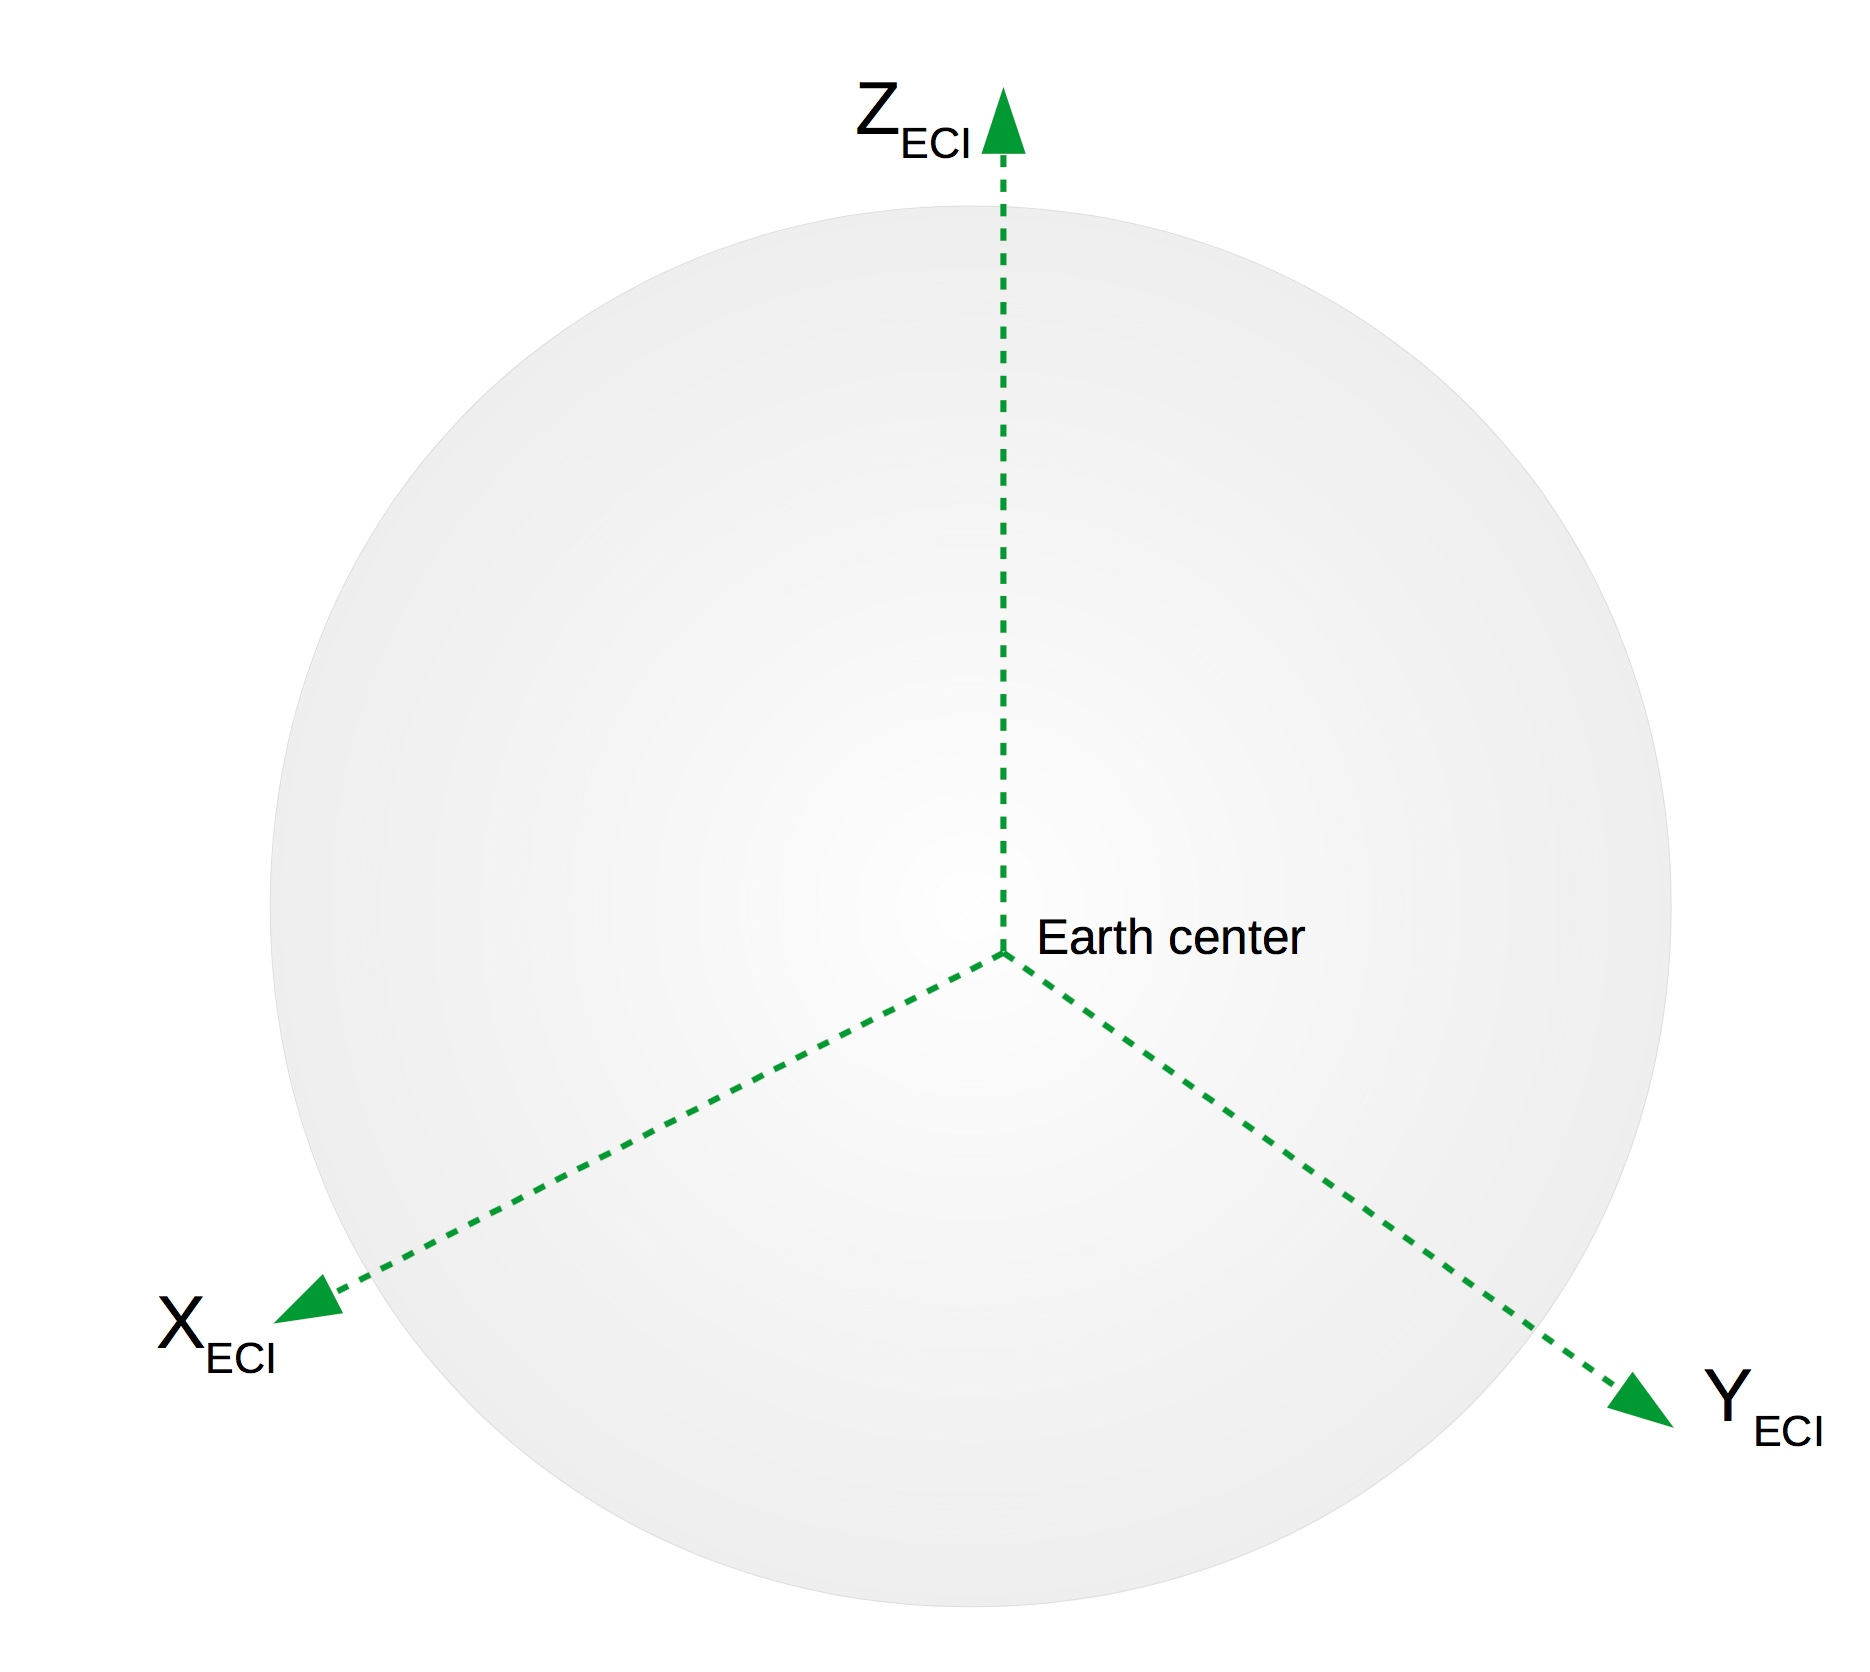
\includegraphics[width=0.5\linewidth]{figures/ECI}
	\caption{ECI coordinate frame}
	\label{fig:ECI}
\end{figure}
\subsubsection{\textit{Earth Centered Earth Fixed Frame (ECEF)}}
Another coordinate frame is the Earth Centered Earth Fixed (ECEF) coordinate frame shown in \figref{fig:ECEF}. In this case the X-axis is passing through the zero longitude, also known as Greenwich meredian, and the Z-axis parallel with the rotational axis. In this way the ECEF frame is fixed to the earth itself and rotates around with it.
\begin{figure}[H]
\centering
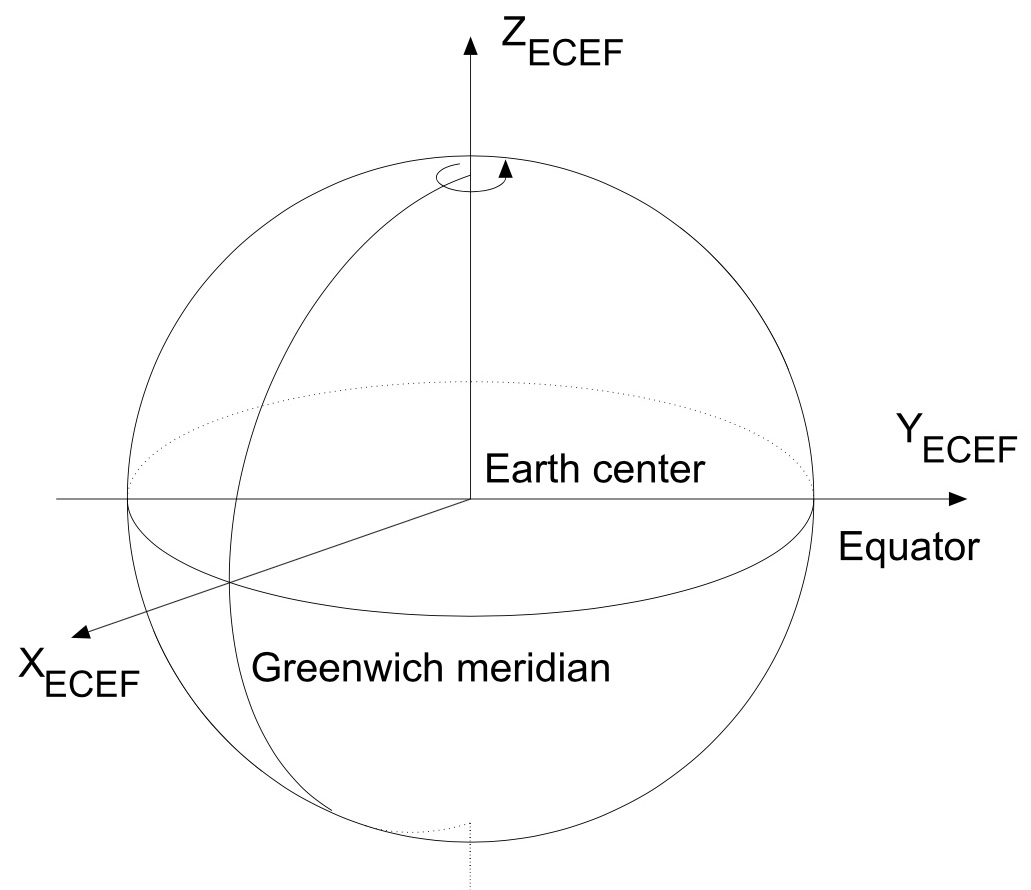
\includegraphics[width=0.5\linewidth]{figures/ECEF}
\caption{ECEF coordinate frame}
\label{fig:ECEF}
\end{figure}
\subsection{Satellite Coordinate Systems}
For the purpose of determining the attitude of the satellite, several coordinate systems are introduced. The attitude and position of the satellite is given as a rotation between the satellite fixed coordinate frames and the reference frames.
\subsubsection{\textit{Orbit Reference frame(ORF)}}
The orbit reference shown in \figref{fig:OFR} is a frame defined in Cartesian coordinates that can be seen as a non-changing frame with respect the earth and the satellite. The $z$ axis always pointing at the Nadir point and it is parallel to the $z_{e}$ axis o the inertial frame of the earth. The $x_{o}$ axis, it is parallel to the orbit plane and $y_{o}$ is the cross product of the $x_{o}$ and $z_{o}$. 
\begin{figure}[H]
	\centering
	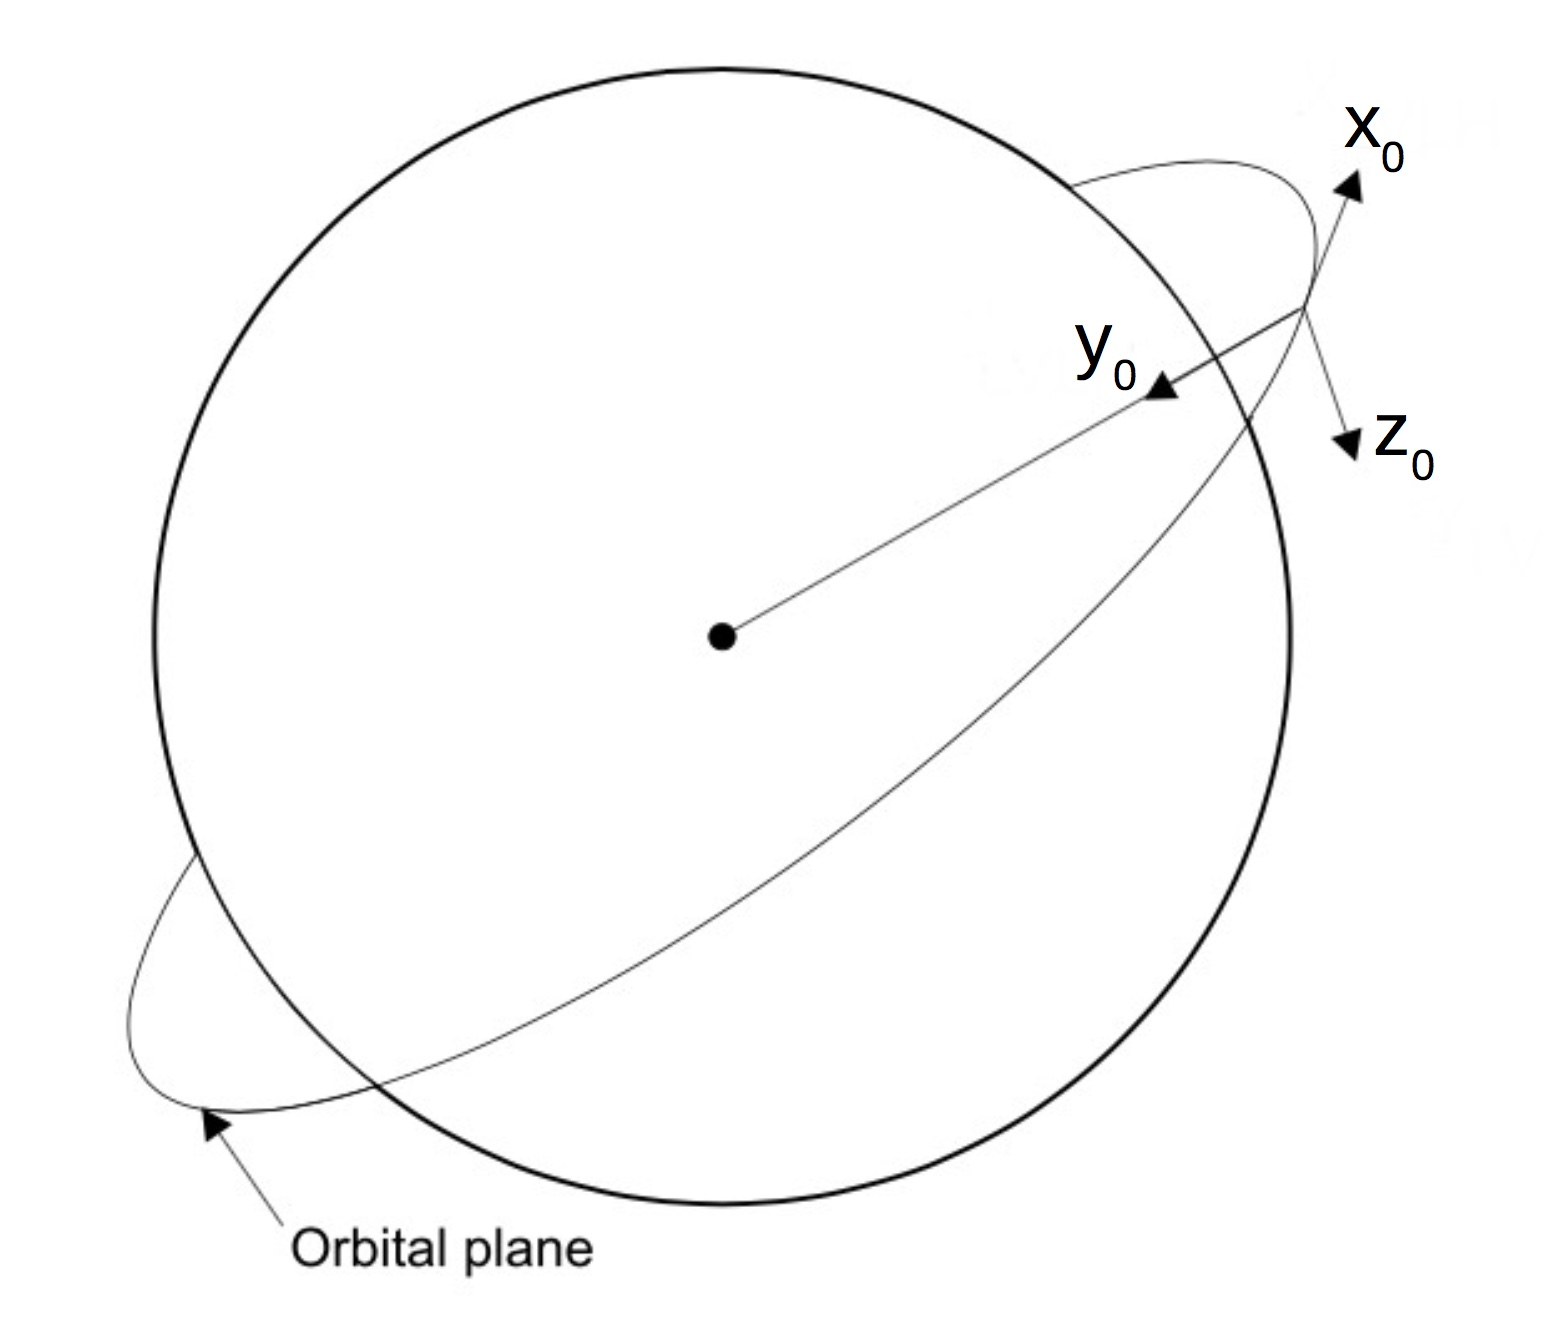
\includegraphics[width=0.4\linewidth]{figures/OFR}
	\caption{ORF coordinate frame}
	\label{fig:OFR}
\end{figure}
\subsubsection{\textit{Satellite Body Frame(SBF)}}
\subsubsection{\textit{Satellite Controller frame(SCF)}}
In order to derive the kinematic equations, a controller reference frame should be specified. It is located in the center of mass of the satellite and it is defined such that the axis of higher inertia $z_{c}$ pointing in the center of ECI and the $x_{c}$ axis with the smallest inertia, pointing along with  the orbit's $x_{o}$ 
\section{Kinematics}
This section will provide the orbit-attitude determination of the satellite using quaternion representation. Since the differential drag control method is based on the rotation of the satellite in order to achieve the effective cross-sectional area, a notation with respect the collaborating frames should be obtained.     
%
\section{Dynamic Model}
In order to describe the behavior of the satellite a dynamic model based on reaction wheels and by using Euler's equation of motion has been derived.   
%
Euler's equation of motion describing the rotation of a rigid body is given by: \fxnote {ref}
% 
\begin{flalign}
	\dot{L} = {N_{tot}- \omega }{\times {L}}
	\label{eq:eulerequation}
\end{flalign}
% 
where $N_{tot}$ represents all the external torques caused from the actuator and the disturbances, $\omega$ is the angular velocity of the satellite and $L$ is the total angular momentum of the satellite and the reaction wheels, given by:
%
\begin{flalign}
	{L} = {I_{s}}{\omega}+{h_{tot}}
	\label{eq:angularmomentum}
\end{flalign}
%
where $h_{tot}$ is the vector of the angular momentum of the wheels $[h_{1} h_{2} h_{3}]^{T}$, all seen in the satellites coordinate system and $I_{s}$ is the inertia matrix of the satellite.
%
Inserting the equation \eqref{eq:angularmomentum} into \eqref{eq:eulerequation} we obtain
%
\begin{flalign}
	{\frac{d}{dt}(I_{s}{\omega})+\dot{h}_{(tot)}} ={N_{tot}-\omega}     {\times  ({I_{s}}{\omega} +{h_{tot}})}
	\label{eq:angularmomentum2}
\end{flalign}
For three reaction wheels attached at the body coordinate system which are the axis roll, pitch and yaw, three equations shall be derived. The derivation of the three equations of motion along with the diagonal inertia matrix can be found in the \label{Appendix A}.      
%
For the ease of notation, the cross product can be written as matrix operation using the $S()$ representing the skew symmetric matrix. Solving for $\dot{\omega}$ the dynamic equation can be written as 
%
\begin{flalign}
	{\dot{\omega}}={-I_{s}^{-1}S(\omega)I_{s}^{-1}\omega-I_{s}^{-1}S(\omega)h_{tot}-I_{s}^{-1}\dot{h}_{(tot)}+I_{s}^{-1}N_{tot}}
	\label{eq:angularmomentum3}
\end{flalign} 
%
The rate of change in angular momentum $\dot{h_{tot}}$ can be absorbed from the controller. This can be written as:
%
\begin{flalign}
	{\dot{h}_{(tot)}} ={-N{c}}
	\label{eq:rate of change}
\end{flalign}
%
where the negative sign denotes the absorbed momentum. The total torque from external disturbances can be written as $N_{dis}$. Rearranging, equation \eqref{eq:angularmomentum3} now reads 
%
\begin{flalign}
	{\dot{\omega}(t)} ={-I_{s}^{-1}S(\omega)I_{s}\omega(t)-I_{s}^{-1}S(\omega)h_{tot}+I_{s}^{-1}N_{c}(t)+I_{s}^{-1}N_{dis}(t)}
	\label{eq:angularmomentum4}
\end{flalign}
%
which constitute the dynamics of the satellite with three reaction wheels. At the final equation \eqref{eq:angularmomentum4} is shown the time dependency of the variables. 
%
\section{Disturbance Models}\label{sec:useCase} 
\subsection{Gravitational torque}
An unbalanced satellite in orbit is subjected to a torque due to the gravitational torque. Assumed that the earth is a point mass and the satellite is a rigid body, the gravitational torque can be estimated. Each infinitesimal element of the satellite of mass \textit{$dm_i$} is subjected to an infinitesimal force \textit{$dF_i$} that can be calculated thanks to Newton's law of universal gravitation.
\[
dF_i = -G\frac{m_{earth}}{R_i^2}dm_i \cdot \hat{R_i}
\]
where \textit{G} is the gravitational constant, \textit{$m_{earth}$} is the mass of the earth and \textit{$R_i^2$} is the vector from the earth to the infinitesimal element of the satellite. \\
The moment of the gravitational force about the geometric center is calculated as the formula:
\[
N_{gra} = \int_{sat} r_i \times dF_i 
\]
with $r_i$ is the vector from the geometric center to the infinitesimal element. $r_i$ can be written as the sum of the vector from the geometric vector to the mass center $r_{g,m}$ and the vector from the mass center of the element $r_{m,i}$. Therefore, the expression of the gravitational torque is simplified:
\begin{align*}
	N_{gra} &= \int_{sat} r_{g,m} \times dF_i + \int_{sat} r_{m,i} \times dF_i \\
	&= \int_{sat} r_{g,m} \times -G\frac{m_{earth}}{R_i^2}dm_i \cdot \hat{R_i} + \int_{sat} r_{m,i} \times -G\frac{m_{earth}}{R_i^2}dm_i \cdot \hat{R_i}
\end{align*}
We can assumed that $r_{m,g} << R_i$ and $R_i$ can be supposed constant and equals to the vector from the center of the earth to the geometric center of the satellite $R_{e,g}$. Thus, The second term is null by definition of the mass center.
\[
\Rightarrow N_{gra} = G\frac{m_{sat} \cdot m_{earth}}{R_{e,g}^2} \cdot (\hat{R_i} \times r_{g,m})
\]
The position of the center of mass was measured for the previous project and is eqals to [?;?;?] in the frame of the satellite. Therefore, $r_{g,m,i}$ can be expressed in the inertial frame as following:
\[
[r_{g,m,i};0] = q_{i,s} \otimes [?;?;?.0] \otimes q_{i,s}*
\]
where $q_{i,s}$ is the quaternion that represents the rotation of the satellite in the inertia frame and $\otimes$ is the quaternion multiplication. Thus, the moment of force can be calculated by this expression above.
  7890